%%%%%%%%%%%%%%%%%%%%%%%%%%%%%%%%
\subsection{Neutrinos in the early Universe}
\label{sec:model:ind}
%%%%%%%%%%%%%%%%%%%%%%%%%%%%%%%%

%%%%%%%%%%%%%%%%%%%%%%%%%%%%%%%%%%%%%%%
\para{Instantaneous Freeze-out Model}
Neutrino freeze-out\index{neutrino!freeze-out} is, as far as we know, the unique era in the history of the Universe when a significant matter fraction froze out at the same time that a reheating period was beginning due to the onset of the $e^+e^-$ annihilation process. It is this coincidence involving the last reheating period that makes neutrino freeze-out a rich and complicated period to study as compared to the many other reheating periods in the history of the Universe. \index{neutrino!freeze-out}


We introduce the effective number of neutrinos\index{neutrino!effective number}, $N^{\text{eff}}_\nu$. This quantity quantifies the amount of radiation energy density, $\rho_r$, in the Universe prior to photon freeze-out and after $e^\pm$ annihilation. $N^{\text{eff}}_\nu$ is a key cosmological observable that can be measured by fitting to the distribution of CMB\index{CMB} temperature fluctuations. The early Planck~\cite{Planck:2013pxb} analysis found $N^{\text{eff}}_{\nu}=3.36\pm 0.34$ (CMB only) and $N^{\text{eff}}_{\nu}=3.62\pm 0.25$ (CMB+$H_0$) ($68\%$ confidence levels), indicating a possible tension in the current understanding of $N^{\text{eff}}_\nu$ though this tension has lessened with further analysis from Planck~\cite{Planck:2015fie,Planck:2018vyg} This section, as well as in Section \ref{ch:param:studies}, works towards a detailed understanding of $N^{\text{eff}}_{\nu}$ with an eye towards this tension.

Mathematically, $N^{\text{eff}}_\nu$ is defined by the relation\index{neutrino!effective number}
\begin{align}\label{eq:NeffDef}
\rho_r=\left(1+(7/8)R_\nu^{4}N^{\text{eff}}_\nu\right)\rho_\gamma\,,
\end{align}
where $\rho_r$ is the radiation component of the Universe energy density, $\rho_\gamma$ is the photon energy density and $R_\nu\equiv T_\nu/T_\gamma=({4}/{11})^{1/3}$ is the photon to neutrino temperature ratio in the limit where the annihilating $e^\pm$ pairs do not transfer any entropy to Standard Model (SM) left-handed neutrinos, i.e., under the assumption that neutrinos have completely frozen out at the time of $e^\pm$ annihilation. The factor 7/8 is the ratio of Fermi to Bose reference normalization in $\rho$ and the neutrino to photon temperature ratio $R_\nu$ is the result of the transfer of $e^\pm$ entropy into photons after neutrino freeze-out\index{neutrino!freeze-out}. 

The definition \ref{eq:NeffDef} is constructed such that if photons and SM left-handed neutrinos are the only significant massless particle species in the Universe between the freeze-out of left-handed neutrinos at $T_\gamma=\mathcal{O}(1)$ MeV and photon freeze-out at $T_\gamma=0.25$ eV, and assuming zero reheating of neutrinos, then $N^{\text{eff}}_{\nu}=3$, corresponding to the number of SM neutrino flavors. Detailed numerical study of the neutrino freeze-out process within the SM gives $N^{\text{eff}}_{\nu}=3.046$~\cite{Mangano:2005cc}, a value close to the number of flavors, indicating only a small amount of neutrino reheating. 
 We emphasize that $N^{\text{eff}}_\nu$ is named after neutrinos as they are the only significant contributor in SM cosmology. However, $N^{\text{eff}}_\nu$ could be impacted by non SM particles.

First we study how $N^{\text{eff}}_{\nu}$ is impacted by non-SM neutrino dynamics by characterizing its dependence on the neutrino freeze-out temperature within an instantaneous freeze-out model. This model, based on the work in \cite{Birrell:2013gpa,Birrell:2012gg}, allows us study $N^{\text{eff}}_{\nu}$ without requiring a detailed description of the underlying non-SM interactions; the latter will be considered later in Section \ref{ch:param:studies}. In addition, we explore the possibility of non-SM neutrino contributions to $N^{\text{eff}}_\nu$; the latter is based on \cite{Birrell:2014cja}.


%%%%%%%%%%%%%%%%%%%%%%%%%%%%
\para{Chemical and Kinetic Equilibrium}
As the Universe expands and cools, the various components of the Universe transition from equilibrium to non-interacting. This process is governed by two key temperatures: 1) The chemical freeze-out temperature, $T_{ch}$, above which the particles are kept in chemical equilibrium\index{chemical equilibrium} by number changing interactions. 2) The kinetic freeze-out temperature, above which the particles are kept in thermal equilibrium, i.e., equilibrium momentum distribution. In reality, these are not sharp transitions, but we approximate them as such in this section. The insights gained here will be important when studying the more detailed model of neutrino freeze-out in later sections.

At sufficiently high temperatures, such as existed in the early Universe, both particle creation and annihilation (i.e., chemical) processes and momentum exchanging (i.e., kinetic) scattering processes can occur sufficiently rapidly to establish complete thermal equilibrium of a given particle species. The distribution function $f_{ch}^\pm$ of fermions (+) and bosons (-) in both chemical and kinetic equilibrium is found by maximizing entropy subject to energy being conserved
\begin{equation}\label{eq:ChEq}
f_{ch}^\pm=\frac{1}{\exp(E/T)\pm 1}\,, \hspace{2mm} T>T_{ch}\,,
\end{equation}
where $E$ is the particle energy, $T$ the temperature, and $T_{ch}$ the chemical freeze-out temperature. 

As temperature decreases, there will be a period where the temperature is greater than the kinetic freeze-out temperature, $T_k$, but below chemical freeze-out. During this period, momentum exchanging processes continue to maintain an equilibrium distribution of energy among the available particles, which we call kinetic equilibrium, but particle number changing processes no longer occur rapidly enough to keep the equilibrium particle number yield, i.e., for $T<T_{ch}$ the particle number changing processes have `frozen-out'. In this condition the momentum distribution, which is in kinetic equilibrium but chemical nonequilibrium, is obtained by maximizing entropy subject to particle number and energy constraints and thus two parameters appear\index{kinetic equilibrium}\index{fugacity}
\begin{equation}\label{eq:kEq}
f_{k}^\pm=\frac{1}{\Upsilon^{-1} \exp(E/T)\pm 1}\,,\hspace{2mm} T_k<T\leq T_{ch}\,.
\end{equation}
The need to preserve the total particle number within the distribution introduces an additional parameter $\Upsilon$ called fugacity. 

The fugacity, $\Upsilon(t)\equiv e^{\sigma(t)}$, controls the occupancy of phase space and is necessary once $T(t)<T_{ch}$ in order to conserve particle number. A fugacity different from $1$ implies an over-abundance ($\Upsilon>1$) or under-abundance ($\Upsilon<1$) of particles compared to chemical equilibrium and in either of these situations one speaks of chemical nonequilibrium. 

The effect of $\sigma$ is similar after that of chemical potential\index{chemical potential} $\mu$, except that $\sigma$ is equal for particles and antiparticles, and not opposite. This means $\sigma>0$ ($\Upsilon>1$) increases the density of both particles and antiparticles, rather than increasing one and decreasing the other as is common when the chemical potential is associated with conserved quantum numbers. Similarly, $\sigma<0$ $(\Upsilon<1)$ decreases both. The fact that $\sigma$ is not opposite for particles and antiparticles reflects the fact that both the number of particles and the number of antiparticles are conserved after chemical freeze-out, and not just their difference. Ignoring the small particle antiparticle asymmetry their equality reflects the fact that any process that modifies the distribution would affect both particle and antiparticle distributions in the same fashion. Such an asymmetry would be incorporated by replacing $\Upsilon\rightarrow \Upsilon e^{\pm\mu/T}$ where $\mu$ is the chemical potential, but we ignore it in this work as the matter antimatter asymmetry is on the order of $1$ part in $10^9$.

 We also emphasize that the fugacity is time dependent and not just an initial condition. At high temperatures $\Upsilon=1$ and we will find that $\Upsilon<1$ emerges dynamically as a result of the freeze-out process. The importance of fugacity was first introduced in \cite{Rafelski:1982pu} in the context of quark-gluon plasma. Its presence in cosmology was noted in \cite{Bernstein:1985th,Dolgov:1992wf} but its importance has been largely forgotten and the consequences unexplored in the literature. 




%%%%%%%%%%%%%%%%%%%%%%%%%%%%%%%%%%%%%%%%%%%%%%%
\index{cosmology!FLRW}
\para{Einstein-Vlasov Equation in FLRW Spacetime}
Once the temperature drops below the kinetic freeze-out temperature $T_k$ of a particular component of the Universe, we reach the free streaming period where all particle scattering processes have completely frozen out. The dynamics are therefore determined by the free-streaming\index{free-streaming} Boltzmann-Einstein\index{Boltzmann-Einstein equation} equation, \req{eq:BoltzmannEinstein} with $C[f]=0$, known as the Einstein-Vlasov equation, in a spatially flat FLRW universe.\index{Einstein-Vlasov equation}

Due to the assumed homogeneity and isotropy, the particle distribution function depends on $t$ and $p^0=E$ only and so the Einstein-Vlasov equation becomes\index{free-streaming}
\begin{equation}\label{VEeqFLR}
E\partial_tf+(m^2-E^2)\frac{\partial_ta}{a}\partial_{E}f=0\,.
\end{equation}
The general solution to \req{VEeqFLR} can be found in, {\it e.g.\/}, ~\cite{Choquet-Bruhat:2009xil,Wong:2011ip}:
\begin{equation}
f(t,E)=K(x)\,,\qquad
x\equiv\frac{a(t)^2}{D^2}(E^2-m^2)\,,
\end{equation}
where $K$ is an arbitrary smooth function and $D$ is an arbitrary constant with units of mass. To continue the evolution beyond thermal freeze-out we choose $K$ to match the kinetic equilibrium distribution \req{eq:kEq} at the freeze-out time $t_k$. This is accomplished by setting
\begin{equation}
K(x)=\frac{1}{\Upsilon_\nu^{-1}e^{\sqrt{x+m^2/T_k^2}}+ 1}
\end{equation}
and $D=T_k a(t_k)$. 

The Fermi-Dirac-Einstein-Vlasov (FDEV) distribution function for neutrinos after freeze-out is then\index{Fermi!Einstein-Vlasov distribution}
\begin{equation}\label{eq:NeutrinoDist}
f(t,E)=\frac{1}{\Upsilon_\nu^{-1}e^{\sqrt{(E^2-m^2)/T_\nu^2+m_\nu^2 /T_k^2}}+ 1}\,,
\end{equation}
where 
\begin{equation}\label{eq:TneutrinoDist}
T_\nu(t)=\frac{T_ka(t_k)}{a(t)}\,. 
\end{equation}
We will call $T_\nu$ in \req{eq:TneutrinoDist} the neutrino background temperature, even though the distribution of free streaming particles has a thermal shape only for $m=0$ and hence $T_{\nu}$ will differ from the temperature of the photon background. The shape seen in  \req{eq:NeutrinoDist} describes a gas of neutrinos that is free streaming in an expanding universe following the freeze-out temperature $T_\nu(t_k)=T_k$. 

The energy, pressure, number density, and entropy density\index{entropy!density} of the free-streaming distribution can be computed using \eqref{Tmndef}, \eqref{nmdef}, and \eqref{smdef}\index{free-streaming!energy density}\index{free-streaming!pressure}\index{free-streaming!number density}
\begin{align}
\rho&=\frac{g_\nu}{2\pi^2}\!\int_0^\infty\!\!\!\frac{\left(m_\nu^2+p^2\right)^{1/2}p^2dp }{\Upsilon_\nu^{-1}e^{\sqrt{p^2/T_\nu^2+m_\nu^2/T_k^2}}+ 1}\,,\label{eq:NeutrinoRho}\\[0.2cm]
P&=\frac{g_\nu}{6\pi^2}\!\int_0^\infty\!\!\!\frac{\left(m_\nu^2+p^2\right)^{-1/2}p^4dp }{\Upsilon_\nu^{-1} e^{\sqrt{p^2/T_\nu^2+m_\nu^2/T_k^2}}+ 1}\,,\label{eq:NeutrinoP}\\[0.2cm]
n&=\frac{g_\nu}{2\pi^2}\!\int_0^\infty\!\!\!\frac{p^2dp }{\Upsilon_\nu^{-1}e^{\sqrt{p^2/T_\nu^2+m_\nu^2/T_k^2}}+ 1}\,,\label{eq:NumDensity}\\[0.3cm]
s&=-\frac{g_\nu}{2\pi^2}\!\int_0^\infty\!\!\!H(p^2/T_\nu^2)p^2dp\,,\,\,\,H\equiv K\ln K +(1-K)\ln(1-K)\,,\label{eq:EntropyIntegrand}
\end{align}
where $g_\nu$ is the neutrino degeneracy (not to be confused with the metric factor $\sqrt{-g}=a^3)$.

Comparing these results to the corresponding quantities in Minkowski space, we see that they differ by the replacement $m\rightarrow m T_\nu(t)/T_k$ in the exponential factor {\em only}. Changing variables to $u=p/T_\nu$, one sees that both $n$ and $s$ are proportional to $T_\nu^3$. The neutrino free-streaming temperature, $T_\nu$, is inversely proportional to $a$, hence we see that
\begin{equation}\label{eq:ConstEntropy}
a^3n=\text{constant}\text{ and } a^3s=\text{constant}.
\end{equation}
This proves that the particle number and entropy in a comoving volume are conserved, irrespective of the form of $K$ that defines the shape of the momentum distribution at freeze-out. It should be noted that this conservation of entropy in free-streaming neutrinos relies on the Boltzmann equation model, and its corresponding entropy current\index{entropy!current} \eqref{smdef}, an approximation which may break down in later epochs of the evolution of the Universe. 

%%%%%%%%%%%%%%%%%%%%%%%%%%%%%%%%%% 
\para{Neutrino Fugacity and Photon to Neutrino Temperature Ratio}
The instantaneous freeze-out assumption allows us to use conservation laws in \req{eq_dynamics} to characterize the neutrino fugacity\index{fugacity!neutrino} and temperature in terms of the freeze-out temperature $T_k$. We first outline the physics of the situation qualitatively. For $T_k<T<T_{ch}$, the evolution of the temperature of the common $e^\pm,\gamma,\nu$ plasma and the neutrino fugacity are determined by conservation of comoving neutrino number (since $T<T_{ch}$) and conservation of entropy. As shown above, after thermal freeze-out the neutrinos begin to free-stream and therefore $\Upsilon_\nu$ is constant, the neutrino temperature evolves as $1/a$, and the comoving neutrino entropy and neutrino number are exactly conserved. 

The photon temperature then evolves to conserve the comoving entropy within the coupled system of photons, electrons, and positrons. As annihilation occurs, entropy from $e^+e^-$ is fed into photons, leading to reheating\index{reheating}. We now make this analysis quantitative in order to derive a relation between the reheating temperature ratio and neutrino fugacity\index{fugacity}.

Assuming $T_{ch}\gg m_e$, the entropy in a given comoving volume, $V(t_{ch})$, is the sum of relativistic neutrinos (with $\Upsilon_\nu=1$), electrons, positrons, and photons
\begin{equation}
S(T_{ch})=\left(\frac{7}{8}g_\nu+\frac{7}{8}g_{e^\pm} +g_\gamma \right)\frac{2\pi^2}{45} T_{ch}^3V(t_{ch})\,,
\end{equation}
where $T_1$ is the common neutrino, $e^+e^-$, and $\gamma$ temperature. 

The number of neutrinos and anti-neutrinos in this same volume is
\begin{equation}
\mathcal{N}_\nu(T_{ch})=\frac{3g_\nu}{4\pi^2}\zeta(3)T_1^3V(t_{ch})\,.
\end{equation}
The particle-antiparticle, flavor, and spin-helicity statistical factors are $g_\nu=6$, $g_{e^\pm}=4$, $g_\gamma=2$.

Distinct chemical and thermal freeze-out temperatures lead to a nonequilibrium modification of the neutrino distribution in the form of a fugacity factor $\Upsilon_\nu$ when $T_k<T<T_{ch}$. This leads to the following expressions for neutrino entropy and number at $T=T_k$ in the comoving volume
\begin{align}
S(T_k)=&\left(\frac{2\pi^2}{45}g_\gamma T_k^3+S_{e^\pm}(T_k)+S_{\nu}(T_k)\right)V(t_k)\,,\\
\mathcal{N}_{\nu}(T_k)=&\frac{g_\nu}{2\pi^2}\int_0^\infty \frac{u^2 du}{\Upsilon_\nu^{-1}(T_k)e^u+1}T_k^3V(t_k)\,.\notag
\end{align}

After neutrino freeze-out\index{neutrino!freeze-out} and when $T_{\gamma}\ll m_e$, the entropy in neutrinos is conserved independently of the other particle species and the $e^+e^-$ entropy is nearly all transferred to photons:
\begin{equation}
S_{\gamma}(T_\gamma)=\frac{2 \pi^2}{45}g_\gamma T_{\gamma}^3 V(t).
\end{equation}
 Note that we must now distinguish between the neutrino and photon temperatures.

The conservation laws \req{eq_dynamics} and \req{eq:ConstEntropy} then imply the following relations.
\begin{enumerate}
\item Conservation of comoving neutrino number between chemical and kinetic freeze-out:
\begin{equation}\label{modindeq1}
\frac{T_{ch}^3V(t_{ch})}{T_k^3V(t_k)}=\frac{2}{3\zeta(3)}\int_0^\infty \frac{u^2 du}{\Upsilon_\nu^{-1}(T_k)e^u+1}.
\end{equation}
\item Conservation of the entropy in $e^\pm$, $\gamma$, and neutrinos prior to neutrino freeze-out:
\begin{align}\label{modindeq2}
&\left(\frac{7}{8}g_\nu+\frac{7}{8}g_{e^\pm} +g_\gamma \right)\frac{2\pi^2}{45} T_{ch}^3V(t_{ch})=\\
&\left(S_{\nu}(T_k)+S_{e^\pm}(T_k)+\frac{2\pi^2}{45}g_\gamma T_k^3\right)V(t_k)\,.\notag
\end{align}
\item Conservation of the entropy in $e^\pm$ and $\gamma$ between neutrino freeze-out and $e^\pm$ annihilation:
\begin{equation}\label{modindeq3}
\frac{2 \pi^2}{45}g_\gamma T_{\gamma}^3 V(t)=\left(\frac{2\pi^2}{45}g_\gamma T_k^3+S_{e^\pm}(T_k)\right)V(t_k)\,, \,\,\, T_\gamma\ll \min\{m_e, T_k\}\,.
\end{equation}
\end{enumerate}

These relations allow one to solve for the fugacity, reheating ratio, and effective number of neutrinos\index{neutrino!effective number} in terms of the kinetic freeze-out temperature, irrespective of the details of the dynamics that leads to a particular freeze-out temperature. Specifically, combining \req{modindeq1} and \req{modindeq2} one obtains
\begin{align}
 \frac{S_{\nu}(T_k)/T_k^3+S_{e^\pm}(T_k)/T_k^3+\frac{2\pi^2}{45}g_\gamma }{\left(\frac{7}{8}g_\nu+\frac{7}{8}g_{e^\pm} +g_\gamma \right)\frac{2\pi^2}{45} }=\frac{2}{3\zeta(3)}\int_0^\infty \frac{u^2 du}{\Upsilon_\nu^{-1}(T_k)e^u+1}.
\end{align}

This can be solved numerically to compute $\Upsilon_\nu(T_k)$. One can also use these relations to analytically derive the following expansion for the photon to neutrino temperature ratio after $e^\pm$ annihilation (see \cite{Birrell:2012gg}):
\begin{align}\label{eq:UpsilonRatio}
&\frac{T_\gamma}{T_\nu}=a\Upsilon^{b}\left(1+c\sigma^2+O(\sigma^3)\right),\\
\label{value_a}
&a=\left(1+\frac{7}{8}\frac{g_{e^\pm}}{g_\gamma}\right)^{1/3}=\left(\frac{11}{4}\right)^{1/3}\,,\,\,\,b\approx 0.367\,, \,\,\,c\approx -0.0209\,.\notag
\end{align}

An approximate power law fit was first obtained numerically in \cite{Birrell:2013gpa}. A relation between the fugacity\index{fugacity} $\Upsilon=e^\sigma$ and the effective number of neutrinos \eqref{eq:NeffDef} was also derived in \cite{Birrell:2012gg} using these methods:
\begin{equation}\label{eq:NnuApprox}
N^{\mathrm{eff}}_\nu=\frac{360}{7\pi^4}\frac{e^{-4b\sigma}}{(1+c\sigma^2)^4}\int_0^\infty \frac{u^3}{e^{u-\sigma}+1}du\left(1+O(\sigma^3)\right)\,.
\end{equation}


%%%%%%%%%%%%%%%%%%%%%%%%%%%%%%%%%%%%%%%
\begin{figure}
\centerline{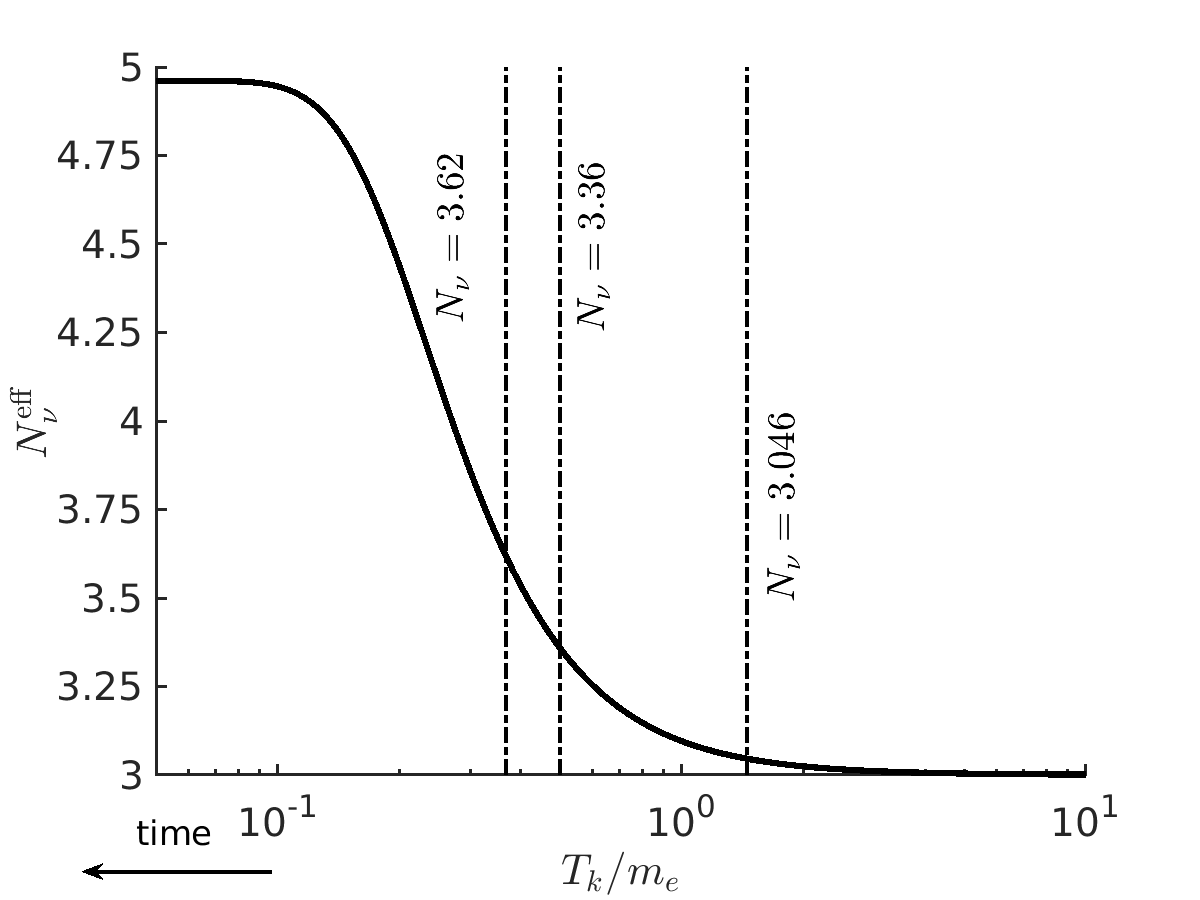
\includegraphics[width=0.90\linewidth]{04-birrell/ModelIndStudy/Figures/N_eff.pdf}}
\centerline{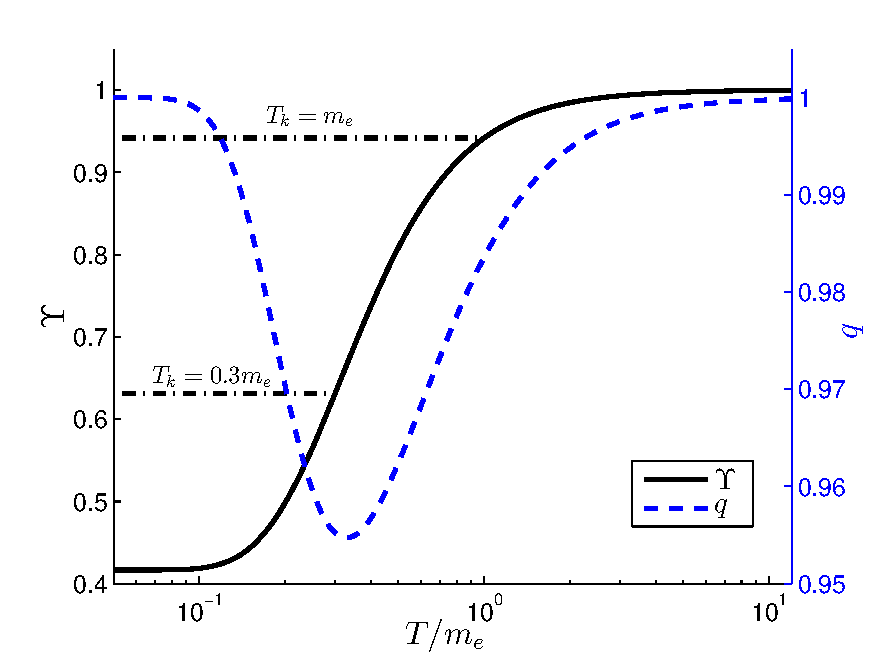
\includegraphics[width=0.90\linewidth]{04-birrell/ModelIndStudy/Figures/Upsilon_q.pdf}}
\caption{Dependence of effective number of neutrinos (top) and neutrino fugacity\index{fugacity!neutrino} (bottom) on the neutrino kinetic freeze-out temperature. We also show the evolution of the deceleration parameter through the freeze-out period (bottom)}
\label{fig:Tk_dependence}
\end{figure}
%%%%%%%%%%%%%%%%%%%%%%%%%%%%%%%%%%%%%%%
 In \rf{fig:Tk_dependence} we plot that dependence of $N^{\mathrm{eff}}_\nu$ and $\Upsilon$ on $T_k$ that is implied by these calculations. In particular, the fugacity evolves following the solid black curve in the bottom plot until it reaches the kinetic freeze-out temperature, at which point the neutrinos decouple and $\Upsilon$ remains constant thereafter, as shown in the dashed black curves for two sample values of $T_k$. 
 

 
Planck CMB\index{CMB} results~\cite{Planck:2013pxb} contain several fits based on different data sets which suggest that $N^{\mathrm{eff}}_\nu$ is in the range $3.30\pm 0.27$ to $3.62\pm0.25$ ($68\%$ confidence level). We note more recent Planck CMB analysis can be found in~\cite{Planck:2018vyg}. A numerical computation based on the Boltzmann equation with two body scattering~\cite{Mangano:2005cc} gives to $N_{\nu}^{\rm eff}=3.046$. These values are shown in the vertical lines in the left figure. The tension between the Planck results and theoretical reheating studies motivates our work.

%%%%%%%%%%%%%%%%%%%%%%%%%%%%%%%%%%%%%%%%%%%%%%%%%%%%%%%%%%%%%%%%%%%%
\para{Contribution to effective neutrino number from sub-eV mass sterile Particles}
Moving beyond neutrinos, we now study the effect on $N_\nu^{\text{eff}}$ of non-SM light weakly coupled particle species, referred to here as a sterile particles (SP)\index{sterile particles}. Such hypothetical SPs would behave as `dark radiation'~\cite{Steigman:2013yua} rather than cold dark matter and would therefore impact $N_\nu^{\text{eff}}$ in a similar manner to neutrinos, though potentially with a vastly different freeze-out temperature. This section is adapted from the work in \cite{Birrell:2014cja}.


The possibility that Goldstone bosons, one candidate for SPs, could be mistaken for a fractional contribution to cosmic neutrinos was identified in \cite{Weinberg:2013kea}. Another viable candidate for SPs are sterile neutrinos. It has been shown that three `new' right-handed neutrinos could fully account for the observed tension in the effective number of neutrinos\index{neutrino!effective number}, $N^{\text{eff}}_{\nu}$, if their freeze-out temperature is in the vicinity of the quark gluon plasma (QGP) phase transition~\cite{Anchordoqui:2011nh,Anchordoqui:2012qu}. If SPs originating in the QGP phase transition are interpreted as Goldstone bosons it would imply that in the deconfined phase there is an additional hidden symmetry, weakly broken at hadronization. For example, if this symmetry were to be part of the baryon conservation riddle, then we can expect that these Goldstone bosons will couple to particles with baryon number, and possibly only in the domain where the vacuum is modified from its present day condition. These considerations motivate study of the contribution to 
$N^{\text{eff}}_{\nu}$ of boson or fermion degrees of freedom (DoF) that froze out near to the QGP phase transformation. 

In this study we use the lattice-QCD derived QGP EoS from~\cite{Borsanyi:2013bia} to characterize the relation between $N^{\text{eff}}_{\nu}$ and the number of DoF that froze out at the time that the quark-gluon deconfined phase froze into hadrons near $T=150\MeV$. We work within the instantaneous freeze-out approximation, using the same reasoning that was applied to neutrinos, {\it i.e.\/}, we employ comoving entropy conservation\index{entropy!conservation} along with the facts that frozen-out particle species undergo temperature scaling with $1/a(t)$ and the remaining coupled particles undergo reheating at each $T\simeq m$ threshold, caused by a disappearing particle species transfer entropy into the remaining particles.



We denote by $S$ the conserved `comoving' entropy in a volume element $dV$, which scales with the factor $a(t)^3$. As we are no longer only considering just the neutrino freeze-out\index{neutrino!freeze-out}, here we employ the definition of the effective number of entropy DoF, $g_*^S$, given by
\begin{equation}
S=\frac{2\pi^2}{45}g^S_*T_\gamma^3 a^3\,.
\end{equation} 
For ideal fermion and boson gases
\begin{equation}
g_*^S=\!\!\!\!\sum_{i=\text{bosons}}\!\!\!\!g_i \left(\frac{T_i}{T_\gamma}\right)^3\!\!\!f_i^-+\frac{7}{8}\!\!\!\sum_{i=\text{fermions}}\!\!\!\! g_i \left(\frac{T_i}{T_\gamma}\right)^3\!\!\!f_i^+\,.
\end{equation}
The $g_i$ are degeneracies, $f_i^\pm$ are known functions, valued in $(0,1)$, that turn off the various species as the temperature drops below their mass; compare to the analogous Eqs. (2.3) and (2.4) in~\cite{Blennow:2012de}. 


%%%%%%%%%%%%%%%%%%%%%%%%%%%%%%%%%%%%%%%
\begin{figure}
\centerline{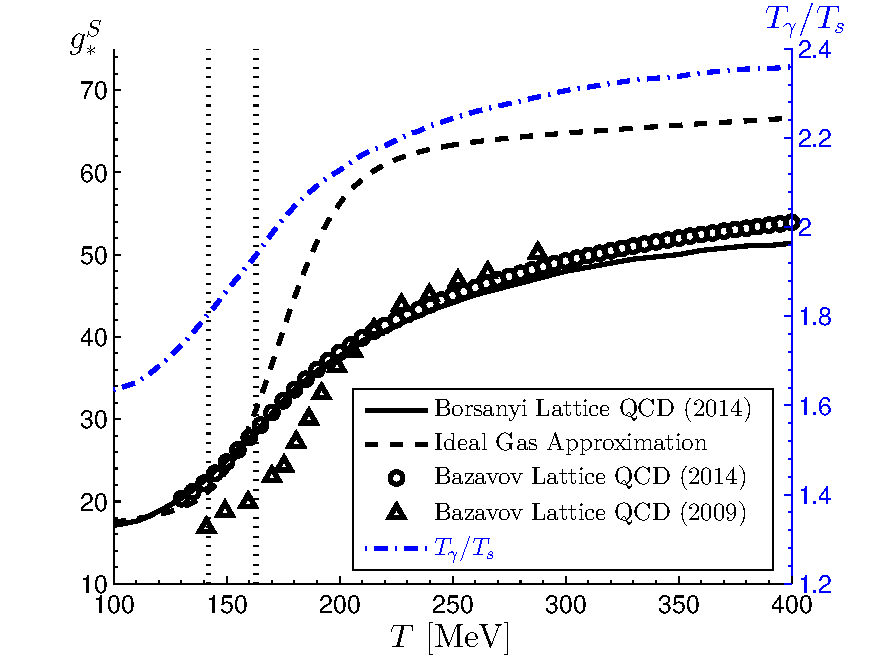
\includegraphics[width=0.9\linewidth]{04-birrell/ModelIndStudy/Figures/gS_T_ratio.pdf}}
\caption{Left axis: Effective number of entropy-DoF, including lattice QCD effects applying~\cite{Borsanyi:2013bia} (solid line) and~\cite{HotQCD:2014kol} (circles), compared to the earlier results~\cite{Bazavov:2009zn} (triangles) used by~\cite{Anchordoqui:2011nh}, and the ideal gas model of~\cite{Coleman:2003hs} (dashed line) as function of temperature $T$. Right axis: Photon to SP temperature ratio, $T_\gamma/T_s$, as a function of SP decoupling temperature (dash-dotted (blue) line). The vertical dotted lines at $T=142$ and 163 MeV delimit the QGP transformation region. \cccite{Birrell:2014cja}\label{fig:gS}}
 \end{figure}
%%%%%%%%%%%%%%%%%%%%%%%%%%%%%%%%%%%%%%%

Such a simple characterization does not hold in the vicinity of the QGP phase transformation where quark-hadron degrees of freedom are strongly coupled and the system must be studied using lattice QCD. A computation of $g_*^S$ that incorporates the lattice QCD results is shown in the solid line in Figure \ref{fig:gS} (left axis). Specifically, we used the table of entropy density\index{entropy!density} values through the QGP phase transition presented by Borsanyi et al.~\cite{Borsanyi:2013bia}, while circles show recent results from Bazavov et al.~\cite{HotQCD:2014kol}. This should be compared to the use of the ideal gas approximation from~\cite{Coleman:2003hs} together with the fit in~\cite{Wantz:2009it} to interpolate though the QGP phase transition and older (year 2009) lattice data from~\cite{Bazavov:2009zn} (triangles). The free gas approximation has a maximum error of $10\%$ in the QGP phase transition temperature range $T\simeq 150$\,MeV. The 2009 lattice data used in~\cite{Anchordoqui:2011nh} has a maximum error on the order of $25\%$ which leads to a non-negligible difference in the relation between freeze-out temperature and $N^{\text{eff}}_{\nu}$.

%%%%%%%%%%%%%%%%%%%%%%%%%%%%%%%%%%%%%%%
\begin{figure} 
\centerline{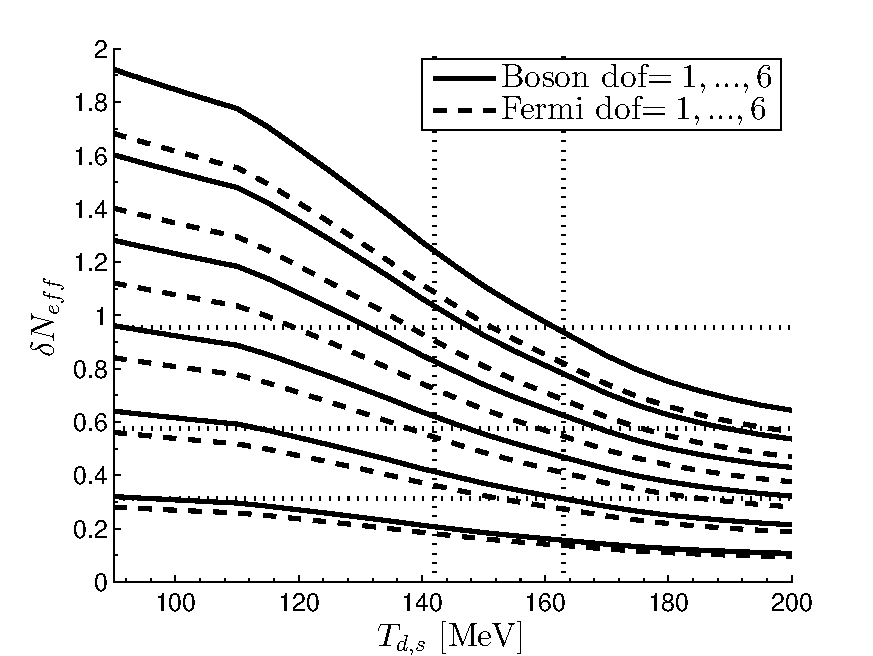
\includegraphics[width=0.9\linewidth]{04-birrell/ModelIndStudy/Figures/Neff_Td_combined.pdf}}
\caption{Solid lines: Increase in $\delta N_{\text{eff}}$ due to the effect of $1,\dots,6$ light sterile boson DoF ($g_s=1,\dots,6$, bottom to top curves) as a function of freeze-out temperature $T_{d,s}$. Dashed lines: Increase in $\delta N_{\text{eff}}$ due to the effect of $1,\dots,6$ light sterile fermion DoF ($g_s=7/8\times 1,\dots,7/8\times 6$, bottom to top curves) as a function of freeze-out temperature $T_{d,s}$. The horizontal dotted lines correspond to $\delta N_{\text{eff}}+0.046=0.36,0.62,1$. The vertical dotted lines show the reported range of QGP transformation temperatures $T_c=142-163\MeV$. \cccite{Birrell:2014cja}\label{fig:NeffTdZoom}}
\end{figure}
%%%%%%%%%%%%%%%%%%%%%%%%%%%%%%%%%%%%


Independent of their source, once the SPs decouple from the particle inventory at a photon temperature of $T_{d,s}$, a difference in their temperature from that of photons will build up during subsequent photon reheating periods, similarly to earlier computations. Conservation of entropy leads to a temperature ratio at $T_\gamma<T_{d,s}$, shown in the dot-dashed line in Figure \ref{fig:gS} (right axis), given by
\begin{equation}\label{eq:TRatio}
R_s\equiv T_{s}/T_{\gamma}=\left(\frac{g_*^S(T_\gamma)}{g_*^S(T_{d,s})}\right)^{1/3}\,.
\end{equation}
Evolving the Universe through neutrino freeze-out\index{neutrino!freeze-out}, if $T_s$ and $T_\gamma$ are the light SP and photon temperatures, both after $e^\pm$ annihilation, and $g_s$ is the number of DoF of the SPs normalized to bosons (i.e., for fermions it includes an additional factor of $7/8$) then this leads to the following change in the effective number of neutrinos\index{neutrino!effective number} in excess of the SM value:
\begin{equation}\label{Neff1}
\delta N_{\text{eff}}\equiv N^{\text{eff}}_{\nu}-3.046=\frac{4g_s}{7}\left(\frac{T_s}{R_s T_{\gamma}}\right)^4\,,
\end{equation}
where $3.046$ is the SM neutrino contribution. Using \req{eq:TRatio} we can rewrite $\delta N_{\text{eff}}$ as
\begin{equation}\label{eq:deltaN}
\delta N_{\text{eff}}=\frac{4g_s}{7R_\nu^4}\left(\frac{g_*^S(T_{\gamma})}{g_*^S(T_{d,s})}\right)^{4/3}\,,
\end{equation}
where $T_{d,s}$ is the decoupling temperature of the SP and $T_{\gamma}$ is any photon temperature in the regime $T_{\gamma}\ll m_e$. The SM particles remaining (in relevant amounts) at such $T_{\gamma}$ are photons and SM neutrinos, the latter with temperature $R_\nu T_{\gamma}$, and so $g_*^S(T_{\gamma})=2+7/8\times 6\times 4/11$ and (see also Eq.(2.7) in~\cite{Blennow:2012de})
\begin{align}\label{eq:deltaN2}
\delta N_{\text{eff}}\approx&g_s\left(\frac{7.06}{g_*^S(T_{d,s})}\right)^{4/3}\,.
\end{align}

In Figure \ref{fig:NeffTdZoom} we plot $\delta N_{\text{eff}}$ as a function of $T_{d,s}$ for $1,\dots,6$ boson (solid lines) and fermion (dashed lines) DoF. For a low decoupling temperature $T_{d,s}<100$\,MeV a single bose or fermi SP can help alleviate the observed tension in $N^{\text{eff}}_{\nu}$. Within the QGP hadronization\index{hadrons!hadronization} temperature range $T_c=142-163\MeV$ (marked by vertical dotted lines) we see that three boson degrees of freedom or four fermion degrees of freedom are the most likely cases to resolve the tension. If the SPs froze out in the QGP phase at $T_{d,s}\gg 163\MeV$ then a significantly larger number of SPs would be required. While such a scenario cannot be excluded, such a large number undiscovered weakly broken symmetries, or/and sterile neutrino-like particles, seems unlikely. Therefore we suggest that Figure \ref{fig:NeffTdZoom} pinpoints the QGP temperature range and below as the primary domain of interest for the freeze-out of a small to moderate number of hypothetical degrees of freedom, should these be responsible the excess in $N_\nu^{\text{eff}}$ above the SM value.
